\documentclass[a4paper, 11pt]{article}

\usepackage[left=1.5cm, right=1.5cm, top=2cm, bottom=2cm]{geometry}

\usepackage[utf8]{inputenc}
\usepackage[T1]{fontenc}
\usepackage[english]{babel}  
\usepackage{lmodern}

\usepackage{amsmath, amsthm, amssymb}
\usepackage{mathtools}

\newtheorem{innercustomgeneric}{\customgenericname}
\providecommand{\customgenericname}{}
\newcommand{\newcustomtheorem}[2]{%
  \newenvironment{#1}[1]
  {%
   \renewcommand\customgenericname{#2}%
   \renewcommand\theinnercustomgeneric{##1}%
   \innercustomgeneric}
  {\endinnercustomgeneric}
}

\newcustomtheorem{thm}{Theorem}
\newcustomtheorem{lem}{Lemma}
\newcustomtheorem{cor}{Corollary}
\newcustomtheorem{deftn}{Definition}
\newcustomtheorem{prop}{Proposition}
\newcustomtheorem{remark}{Remark}

\DeclareMathOperator*{\argmin}{argmin} 
\DeclareMathOperator*{\argmax}{argmax} 

\renewcommand{\thesection}{\Roman{section}} 

\begin{document}
\title{Hermite Polynomials snakes order 2}
\author{Yoann Pradat}
\maketitle

\section{Translation of Schoenberg's 1973 paper for the case $r=3, m=3$}

The following is simply a reminder of some of the results found by I.J Schoenberg in his paper \emph{Cardinal 
Interpolation and Spline Functions. III Cardinal Hermite interpolation}. Let's reintroduce notations of the article and 
make somehow more explicits what the objects they encode are. \\

Let $r$ and $m$ be positive integers that satisfy $r \leq m$. The set of cardinal splines of order $2m$ with knot 
multiplicity $r$ is denoted by $S_{2m,r}$. Note that using De Boor's notations for splines set we have the following

\begin{equation}
  S_{2m,r} = \$_{2m, \mathbb{Z}_3} = \Pi_{< 2m, \mathbb{Z}, 2m-r}
\end{equation}

where $\mathbb{Z}_{3}$ denotes the sequence of knots $(\dots, -1,-1,-1, 0, 0, 0, 1, 1, 1, \dots)$. It is clear from 
these notations that $S_{2m, r} \subset \mathcal{C}^{2m-r-1}$. 

\begin{thm}{1}
  Let $S$ be either of the vector spaces $\mathcal{L}_{p,r}, F_{\gamma,r}$ with $\gamma \geq 0$, $p \in \mathbb{N}^*$.  
  Provided a solution to C.H.I.P $\left( y_{\nu}, \dots,  y_{\nu}^{(r-1)}, S_{2m,r} \cap S \right)$ exists, it is 
  uniquely given by
  \begin{equation}
    \forall x \in \mathbb{R} \qquad S(x) = \sum_{\nu = - \infty}^{\infty} y_{\nu} L_0(x-\nu) + \cdots + y_{\nu}^{(r-1)} 
    L_{r-1}(x-\nu)
  \end{equation}
\end{thm}

In order to specify a usable model for active contours it remains to determine explicit expressions for the basis 
functions $L_0, \dots, L_{r-1}$. In the article they are determined by solving a set of $2m-r$ linear equations. This 
system is obtained by considering separately the function $L_s$ on $[1, \infty)$ and $[0,1]$. Note that specifying the 
function on both these intervals completely determine $L_s$ as the latter is even (if $s$ is even) or odd (if $s$ is 
odd). \\  

On $[1,\infty)$, $L_s$ can be decomposed into 

\begin{equation*}
  L_s = \sum_{j=1}^{m-r} c_j S_j
\end{equation*}

where $(c_j)_{j=1}^{m-r}$ are $(m-r)$ unknown coefficients to be determined and $S_j$ are the eigensplines for the first 
$m-r$ “eigenvalues” $\lambda_j$, solutions to $|\Delta_{r,d}(\lambda)|=0$. \\

On $[0,1]$, $L_s$ is given by a polynomial $P$ of order $2m$ that takes a specific form according to the parities of $s$ 
and $r$ (we refer to equations (7.13) and (7.14)) in the article. This polynomial introduces $m$ unknown coefficients 
$(a_j)_{j=1}^{m}$. To determine a total of $m + m-r = 2m-r$ unknown coefficients we make use of the $2m-r$ equality 
conditions at 1 $P^{(\rho)}(1) = L_s^{(\rho)}(1)$. We end up of a system of $2m-r$ equations for $2m-r$ unknowns that 
can be solved exactly provided the matrix of the system is non singular. Schoenberg proves with a very nice argument 
that the matrix of the system is always non singular. \\

\clearpage

In the case $m=r=3$, $L_0, L_1, L_2$ are 0 on $[1, \infty)$ and on $[0,1]$ are given by 

\begin{align}
  L_0(x) &= 1 + a_1 x^3 + a_2 x^4 + a_3 x^5 \\
  L_1(x) &= x + a_1 x^3 + a_2 x^4 + a_3 x^5 \\
  L_2(x) &= \frac{1}{2}x^2 + a_1 x^3 + a_2 x^4 + a_3 x^5
\end{align}

where the coefficients for each generator are unrelated. Note that $L_s$ have finite support \emph{because} $m=r$. If 
that was not the case the term $\displaystyle \sum_{j=1}^{m-r} c_j S_j$ may not be 0 and therefore $L_s$ would be non 
zero on $[1, \infty)$! Can it happen though that $m > r$ and $(c_j)_{j=1}^{m-r}$ are 0? To determine the coefficients 
above we need to solve independently for each generator the 3 equations $P^{(\rho)}(1) = 0$. This leads to the following 
systems

\begin{equation*}
  \left\{
  \begin{array}{r @{{}={}} r}
    a_1 + a_2  + a_3 & -1 \\
    3a_1 + 4a_2 + 5a_3 & 0 \\
    3a_1 + 6a_2  + 10a_3 & 0\\
  \end{array}
  \right.
  \hfill
  \left\{
  \begin{array}{r @{{}={}} r}
    a_1 + a_2  + a_3 & -1 \\
    3a_1 + 4a_2 + 5a_3 & -1 \\
    3a_1 + 6a_2  + 10a_3 & 0\\
  \end{array}
  \right.
  \hfill
  \left\{
  \begin{array}{r @{{}={}} r}
    a_1 + a_2  + a_3 & -\frac{1}{2} \\
    3a_1 + 4a_2 + 5a_3 & -1 \\
    3a_1 + 6a_2  + 10a_3 & -\frac{1}{2} \\
  \end{array}
  \right.
\end{equation*}

\section{The resulting snake scheme}

\subsection{Generating functions}

\begin{figure}[!h]
  \centering
  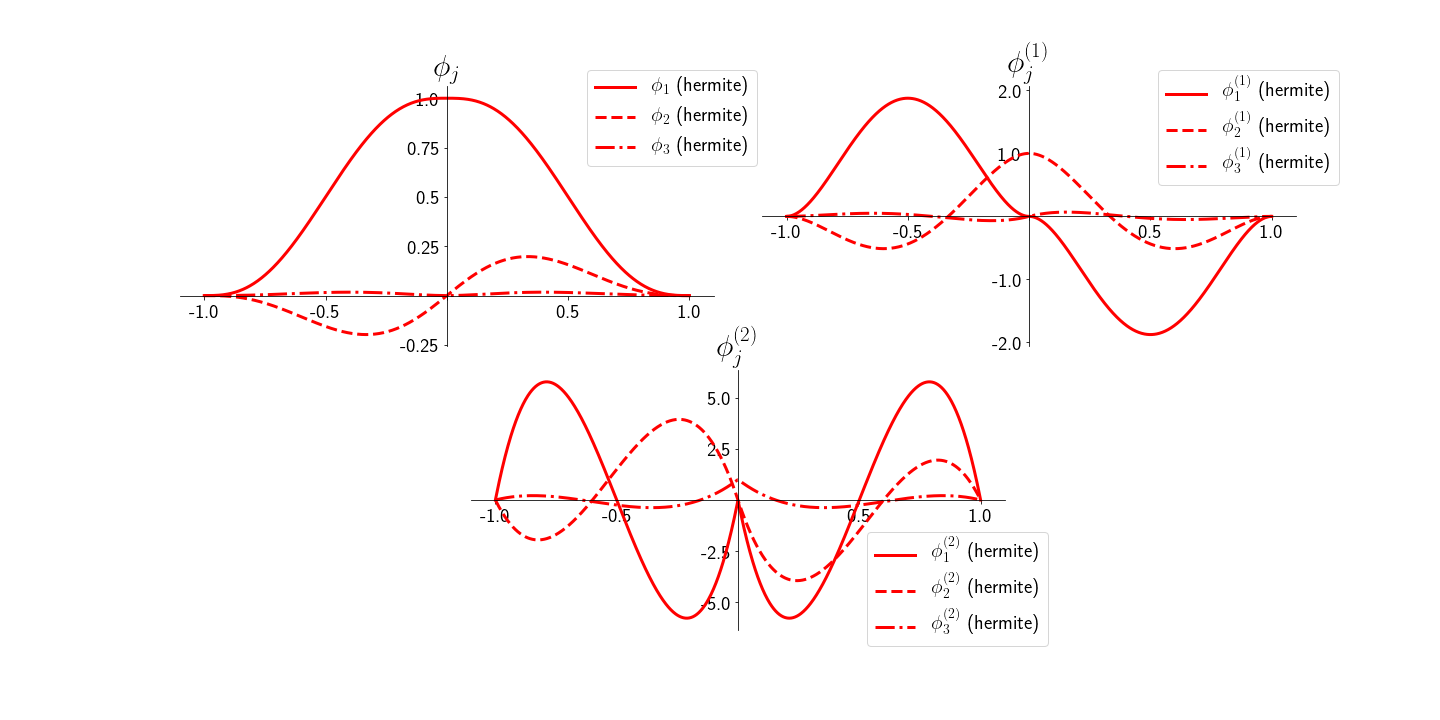
\includegraphics[width=\textwidth]{basis.png}
  \caption{Generators for C.H.I.P with $m=r=3$}
  \label{fig:basis}
\end{figure}


Solving the linear systems written in the previous section yields explicit formulas for the Schoenberg basis generators 
$L_0, L_1, L_2$, that we rename $\phi_1, \phi_2, \phi_3$ in accordance with modern notations (see V. Uhlmann 
\emph{Hermite Snakes with Controls of Tangents}). The formulas are the following. 

\begin{align}
  \phi_1(x) &= \begin{dcases} 
    1 - 10 x^3 + 15 x^4 - 6 x^5 & \text{if } 0 \leq x \leq 1  \\
    1 + 10 x^3 + 15 x^4 + 6 x^5 & \text{if } -1 \leq x < 0 \\
  \end{dcases} \\
  \phi_2(x) &= \begin{dcases}
    x - 6 x^3 + 8 x^4 - 3 x^5 & \text{if } 0 \leq x \leq 1  \\
    x - 6 x^3 - 8 x^4 - 3 x^5 & \text{if } -1 \leq x < 0 \\
  \end{dcases} \\
  \phi_3(x) &= \begin{dcases}
    0.5 x^2 - 1.5 x^3 + 1.5 x^4 - 0.5 x^5 & \text{if } 0 \leq x \leq 1  \\
    0.5 x^2 + 1.5 x^3 + 1.5 x^4 + 0.5 x^5 & \text{if } -1 \leq x < 0 \\
  \end{dcases}
\end{align}

In figure~\ref{fig:basis} are displayed the values of these functions as well as their two first derivatives. As 
mentioned in the previous section, the generators $L_s$ are elements of $S_{2m, r}=S_{6,3}$ which is a subset of 
$\mathcal{C}^{2m-r-1} = C^{2}$. It is apparent in the figure that these functions have continuous derivatives up to 
order 2 but that higher order derivatives do not exist in neighborhoods of $-1, 0$ and $1$.

\subsection{Closed planar curves or “contours”}

Consider a positive integer $M$ and an \textbf{$M$-periodic parametrized closed curve} $r: \mathbb{R} \to \mathbb{R}^2$ 
for which we have local derivatives up to order 2 at $M$ location sites regularly spaced that is we know ${(r[k], r'[k], 
r''[k])}_{k=0}^{M-1}$. 

\begin{cor}{1}
  Given $M$ periodic sequences  ${(r[k], r'[k], r''[k])}_{k \in \mathbb{Z}}$, there exists a unique spline of order $6$ 
  whose value and derivatives agree with the sequence of coefficients at integers locations. This spline and its 
  derivatives are everywhere bounded and take the form for $t \in \mathbb{R}$

\begin{align}
  r(t) &= \sum_{k \in \mathbb{Z}} r[k] \phi_1(t-k) + r'[k] \phi_2(t-k) + r''[k] \phi_3(t-k) \\
  &= \sum_{k=0}^{M-1} r[k] \phi_{1, per}(t-k) + r'[k] \phi_{2, per}(t-k) + r''[k] \phi_{3, per}(t-k) 
  \label{eq:curve_nno}
\end{align}

\end{cor}

\begin{proof}
As the sequence of coefficients ${(r[k], r'[k], r''[k])}_{k \in \mathbb{Z}}$  are in $Y_{\gamma, r} = Y_{0, 3}$ (i.e 
they are bounded), application of Schoenberg's theorem 1 yields existence and unicity of a interpolating function in 
$S_{6,3} \cap F_{0, 3}$. Application of theorem 4 then leads to the explicit formulation given above.
\end{proof}

\begin{remark}{1} It is convenient to normalize the continuous parameter to the $[0,1]$ interval as is usual in the 
  implementations.  For that let the renormalized curve $s(t) = r(Mt)$ for $t \in [0,1]$. Note that this completely 
  describes the curve as it is enough to describe the curve $r$ on $[0,M]$. Differentiating this equality twice yields 
  $r[k] = s[\frac{k}{M}], r'[k] = \frac{1}{M} s'[\frac{k}{M}], r''[k] = \frac{1}{M^2} s''[\frac{k}{M}]$. Therefore 
  equation (\ref{eq:curve_nno}) is rewritten for $t \in [0,1]$

\begin{equation}
  \label{eq:ccurve_no}
  s(t) = \sum_{k=0}^{M-1} s[\frac{k}{M}] \phi_{1, per}(Mt-k) + \frac{1}{M} s'[\frac{k}{M}] \phi_{2, per}(Mt-k) + 
  \frac{1}{M^2} s''[\frac{k}{M}] \phi_{3, per}(Mt-k)
\end{equation}

\end{remark}

In the rest of this document we will reuse the notation $r$ for the normalized curve and won't make use of the notation 
$s$ anymore. Equation (\ref{eq:ccurve_no}) is the \textbf{mathematical representation of a planar curve} and we call it 
“snake” or “active contour”. By playing with the coefficients we can capture a wide variety of contours that arise from 
closed objects in 2D images like cells membrane in a bioimage. 

\subsection{Open planar curves}

Consider again a positive integer $M$ and a \textbf{parametrized open curve} $r: \mathbb{R} \to \mathbb{R}^2$ for which 
we have local derivatives up to order 2 at $M$ location sites regularly spaced that is we know ${(r[k], r'[k], 
r''[k])}_{k=0}^{M-1}$. By “open” we mean a curve that is not periodic. 

\begin{cor}{2}
  Given biinfinite sequences of coefficients $(\dots, 0, r[0], \dots, r[M-1], 0, \dots)$, $(\dots, 0, r'[0], \dots, 
  r'[M-1], 0, \dots)$, $(\dots, 0, r''[0], \dots, r''[M-1], 0, \dots)$there exists a unique spline of order $6$ 
  whose value and derivatives agree with the sequence of coefficients at integers locations. This spline and its 
  derivatives have compact support and take the form for $t \in \mathbb{R}$

  \begin{align*}
    r(t) &= \sum_{k \in \mathbb{Z}} r[k] \phi_1(t-k) + r'[k] \phi_2(t-k) + r''[k] \phi_3(t-k) \\
    &= \sum_{k=0}^{M-1} r[k] \phi_{1}(t-k) + r'[k] \phi_{2}(t-k) + r''[k] \phi_{3}(t-k)
  \end{align*}
\end{cor}

\begin{proof}
  This result is again a simple application of theorem 1 and 4 given in Schoenberg's paper of 1981.
\end{proof}

\begin{remark}{2}
  In this setting we are only interested in the curve lying between our coefficients that is the interpolated points 
  with continuous parameter in the interval $[0, M-1]$  The normalization factor is therefore $M-1$ and the renormalized 
  open curve $s(t) = r((M-1)t)$ takes the form

  \begin{equation}
    \label{eq:ocurve_no}
    s(t) = \sum_{k=0}^{M-1} s[\frac{k}{M-1}] \phi_{1}((M-1)t-k) + \frac{1}{M-1} s'[\frac{k}{M-1}] \phi_{2}((M-1)t-k) + 
  \frac{1}{(M-1)^2} s''[\frac{k}{M-1}] \phi_{3}((M-1)t-k)
  \end{equation}
  which we will also renote $r$.
\end{remark}

\subsection{Closed sphere-like surfaces}

In my research project we are interested in developing a mathematical methods for representing a certain type of 
surfaces with explicit control of local properties including first-order derivatives and curvature. As a consequence 
extension of the schemes given in equations (\ref{eq:ccurve_no}) and (\ref{eq:ocurve_no}) to tensor-product surfaces 
(that is surfaces parametrized by 2 continuous parameters in a way that each continuous parameter appear in separate 
functions) may be relevant for the questions we have. \\ 

Consider positives integers $M_1$ and $M_2$ and a \textbf{sphere-like parametrized} surface $\sigma: U \subseteq 
\mathbb{R}^2 \to \mathbb{R}^3$ with $U$ a subset (closed in our case) of the plane. By “sphere-like” we mean an object 
that can be described with closed curves on latitudes ($u$ varies while $v$ is fixed) and open curves on longitudes ($v$ 
varies while $u$ is fixed). Suppose we have local properties of the surface at $M_1\times(M_2+1)$ locations (counted 
with multiplicity as some locations may coalesce) on a regular grid. \\ 

\begin{cor}{3}
  Given the biinfinite sequences of coefficients $(\partial^{i,j}\sigma(k,l))_{k, l \in \mathbb{Z}^2, (i,j) \in 
  \{0,1,2\}^2}$ that are $M_1$ periodic in the first coordinate and vanish when the second coordinate is outside $[0, 
  M_2]$, there exists a unique interpolating tensor-product spline of order $6$ whose value and partial derivatives 
  agree with the sequence of coefficients at the integers grid locations. This tensor-product spline and its derivatives 
  are everywhere bounded and take the form for $(u,v) \in [0,1]^2$

  \begin{equation}
    \sigma(u,v) = \sum_{k=0}^{M_1-1} \sum_{l=0}^{M_2} \sum_{i,j = 0}^2 \frac{1}{M_1^i M_2^j} \partial^{i,j}
    \sigma(\frac{k}{M_1}, \frac{l}{M_2}) \phi_{i+1, per}(M_1u-k) \phi_{j+1}(M_2v-l)
  \end{equation}
\end{cor}{3}

\begin{proof}
  This is a simple application of corollaries 1 and 2 given before.
\end{proof}




\end{document}
